\documentclass[10pt]{article}
%\usepackage{widetext}
\usepackage{amsmath}
\usepackage{enumerate}
\usepackage{array}
\usepackage{subfig}
\usepackage{graphicx}
\usepackage{float}
%\usepackage[footnotesize,bf]{caption}
%\usepackage{subcaption}
\usepackage{amsfonts}
\usepackage{amssymb}
\usepackage{epstopdf}
\usepackage[cm]{fullpage}
\usepackage{multicol}
\usepackage{multirow}
\usepackage{authblk}
\usepackage{mathtools}
\usepackage{titlesec}
\usepackage{booktabs}
%\usepackage{ amssymb }
\setlength\parindent{0pt}
\setlength{\columnsep}{0.5cm}
\captionsetup[sub]{font=\normalsize}

\titleformat{\section}
  {\normalfont\sffamily\Large\bfseries}
  {\thesection}{0.5em}{}
\titleformat{\subsection}
  {\normalfont\sffamily\large\bfseries}
  {\thesubsection}{0.5em}{}

\newenvironment{Figure}
  {\par\medskip\noindent\minipage{\linewidth}}
  {\endminipage\par\medskip}


\title{Variable population mixing in disease models}
\author[1]{Ewan Colman, Andreas Modlmeier, David Hughes, Shweta Bansal}
\begin{document}
\maketitle
\vspace{-0.7cm}
\begin{abstract}
\noindent\normalsize
How individuals move, interact, and mix in a population is critical to the success of an infectious disease. In this paper we introduce a novel method to quantify the level of mixing in a social system and demonstrate how it contributes to the risk of epidemic outbreak. We develop a dynamic model in which the contact rates between individuals varies heterogeneously across the population. The parameter that controls this heterogeneity, $\phi\geq 0$, also controls the propensity of individuals to mix with other members of the population. By fitting this model to dynamic network data, the mixing parameter can be estimated in various social systems. We use data from food sharing interactions between ants, face-to-face contacts between humans, and online social networks. We examine relationship between the level of mixing and the number of secondary cases caused by an infected individual and find that mixing in a population accelerates the spread of disease. 
\end{abstract}
\vspace{0.5cm}
\begin{multicols}{2}
\section{Introduction}
\noindent
Infectious diseases thrive when they have regular and easy access to susceptible victims. The variety of known diseases show us that this can be achieved in a number of ways. Airborne diseases such as influenza prosper when groups of people or livestock congregate in relatively small spaces \cite{doi:10.1093/oxfordjournals.aje.a112781,koopmans2004transmission}. Pathogens of this type can reach a large number of individuals but have only a small probability of infecting each one \cite{doi:10.1093/infdis/jis773}. Sexually transmitted diseases, on the other hand, compensate for their relative scarcity of opportunities by having a high probability of transmission during intercourse and a slow immune response once the host is infected \cite{anderson1990significance}. 

From these examples it would seem clear that one of two approaches should be applied to model infectious disease. We could treat the system as a well-mixed fluid in which the spread of disease depends solely on the size and density of the population \cite{de1995does,anderson1992infectious}. This is generally known as the mass-action model and is the most established approach to disease modeling \cite{begon2002clarification}. Alternatively we could examine the network of social or sexual relationships and predict how an infection might flow from one node to the next \cite{rothenberg1998using}.

Now consider an ant colony. Through contact ants are able to transmit parasitic fungi, and through trophallaxis (mouth-to-mouth food sharing) a variety of other infections can spread \cite{greenwald2015ant,10.7554/eLife.20375}. Each ant has a role in the society, e.g. forager, nurse etc., and this determines which spatial region in the nest they will occupy \cite{gadau2009organization,Mersch1090}. Infectious interactions are therefore driven in part by chance encounters, and in part by preference to be where their designated role requires them to be. 

Thus, we cannot say that the system is well-mixed and that interactions occur between any random pair of ants, but at the same time we cannot predict where interactions will occur based on the social structure alone. To model disease spread in this context we need an approach that mediates between the network-based disease models and those built on the well-mixed assumption. 

One approach is to consider what happens when edges change over time \cite{Volz2925}. As time progresses, the number of new connections one accumulates will grow at a rate that depends on the rate at which the connections change. As we would expect, higher rates of mixing lead to higher rates of disease transmission and an increased risk of an epidemic outbreak \cite{volz2009epidemic}. While this version of mixing is clearly relevant to disease outcomes, analysis of this model has yet only considered randomly assigned connections, whereas most problems with traditional models result from the fact that social structure is non-random \cite{Bansal879}. 

In studies of human disease this problem is often answered by incorporating a mixing matrix into the disease model, sometimes referred to as a WAIFW (who acquires infection from whom) matrix \cite{anderson1992infectious}. This approach involves partitioning the population into a number of categories, for example by age or gender, then assigning different contact for each different type of interaction \cite{castillo1989epidemiological,DelValle2007539}. This approach can be useful on a large scale but to be applicable in localized settings, such as at a school or workplace, the detail required in order to categorize each individual is much higher. 

In this paper we show that it is possible to analyze mixing in small localized populations without large amounts of personal information, instead we rely on a general theory of human and animal social behavior. We first mention some related literature that motivates our approach to the problem (Section \ref{background}). We model the interactive behavior of individuals in a population by considering their propensity to socially mix (Section \ref{social_mixing}). One parameter in the model, $\phi$, controls the heterogeneity of contact probabilities and we show how it can be tuned to achieve the levels of mixing observed in various human and animal populations (Section \ref{fitting}). 

We then consider how mixing affects the spread of disease (Section \ref{disease_section}). We derive a formula for the expected number of secondary infections originating from one infected host as a function of $\phi$ (for a disease with susceptible $\rightarrow$ infectious $\rightarrow$ removed dynamics), estimate $\phi$ in $25$ dynamic contact networks, and show that mixing is directly related to the number of secondary infections caused (Section \ref{results} and in Figures \ref{Degree_vs_int} and \ref{disease_fig}).

\section{Modeling and analysis}
\subsection{Background}
\label{background}
All social species are driven by an intrinsic need to bond with others. In most cases, the number of social contacts an individual can maintain is constrained by the limitations of time and energy [reference?]. In primates, including humans, it is also restricted by the cognitive capacity of the species \cite{dunbar1998social,10.1371/journal.pmed.1000316,dunbar2014human}. This means individuals are frequently confronted with a choice: to invest in forming new relationships or to invest in maintaining pre-existing ones. Since the second option is usually favored over the first, social networks change at a relatively slow pace.
 
Another result of this is that the distribution of relationship strengths for most people is heterogeneous; most time is invested in close contacts (best friends, family members, etc.), less is invested in the wider friendship circle, and as the circle extends to a wider selection of people, the frequency of interaction decreases \cite{MacCarron2016151,dunbar1998social}. We see the effect of this heterogeneity when we observe an individual over the course of a day (or week, or year) and compare their overall amount of social activity to the number of social connections they made during that time \cite{10.1371/journal.pone.0022656}. Gregarious individuals, for example, are those who engage in a large number of interactions and also have a relatively large set of social contacts. Compared to others they show little preference to interact with one individual over any other, or in other words, they have low heterogeneity in the distribution of their relationship strengths. By answering the question of how such social choices are made, the level of sociality can be modeled and quantified \cite{karsai2014time}.

Since the question of social preference is based only decision making, it can be asked without the need to consider the time-scale on which the social activity occurs. We must, however, be conscious of the role of time in how an interaction is interpreted in the context of transmissible disease. The assumption [choose a better word EC] that we make, and continue to make throughout this paper, is that all interactions carry the same probability of infection $\beta$. We are thus disregarding the fact that interactions vary in duration, intimacy, and contact type; $\beta$ represents a probability of infection that takes all such variables into account.

Thus, each interaction between an infected host and a susceptible contact presents a new opportunity for the disease to transmit. Given this interpretation we can deduce that restrained social behavior helps to mitigate the risks of disease spread; once a disease has spread from one individual to another, repetition of the same interaction presents no advantage for the infectious agent (who would rather its host be interacting with someone unfamiliar and susceptible). Repeated contact with a small number of individuals is therefore, in general, a safer strategy than constantly seeking to interact with less familiar members of the population \cite{karsai2014time}. 

\begin{figure*}[t]
\centering
		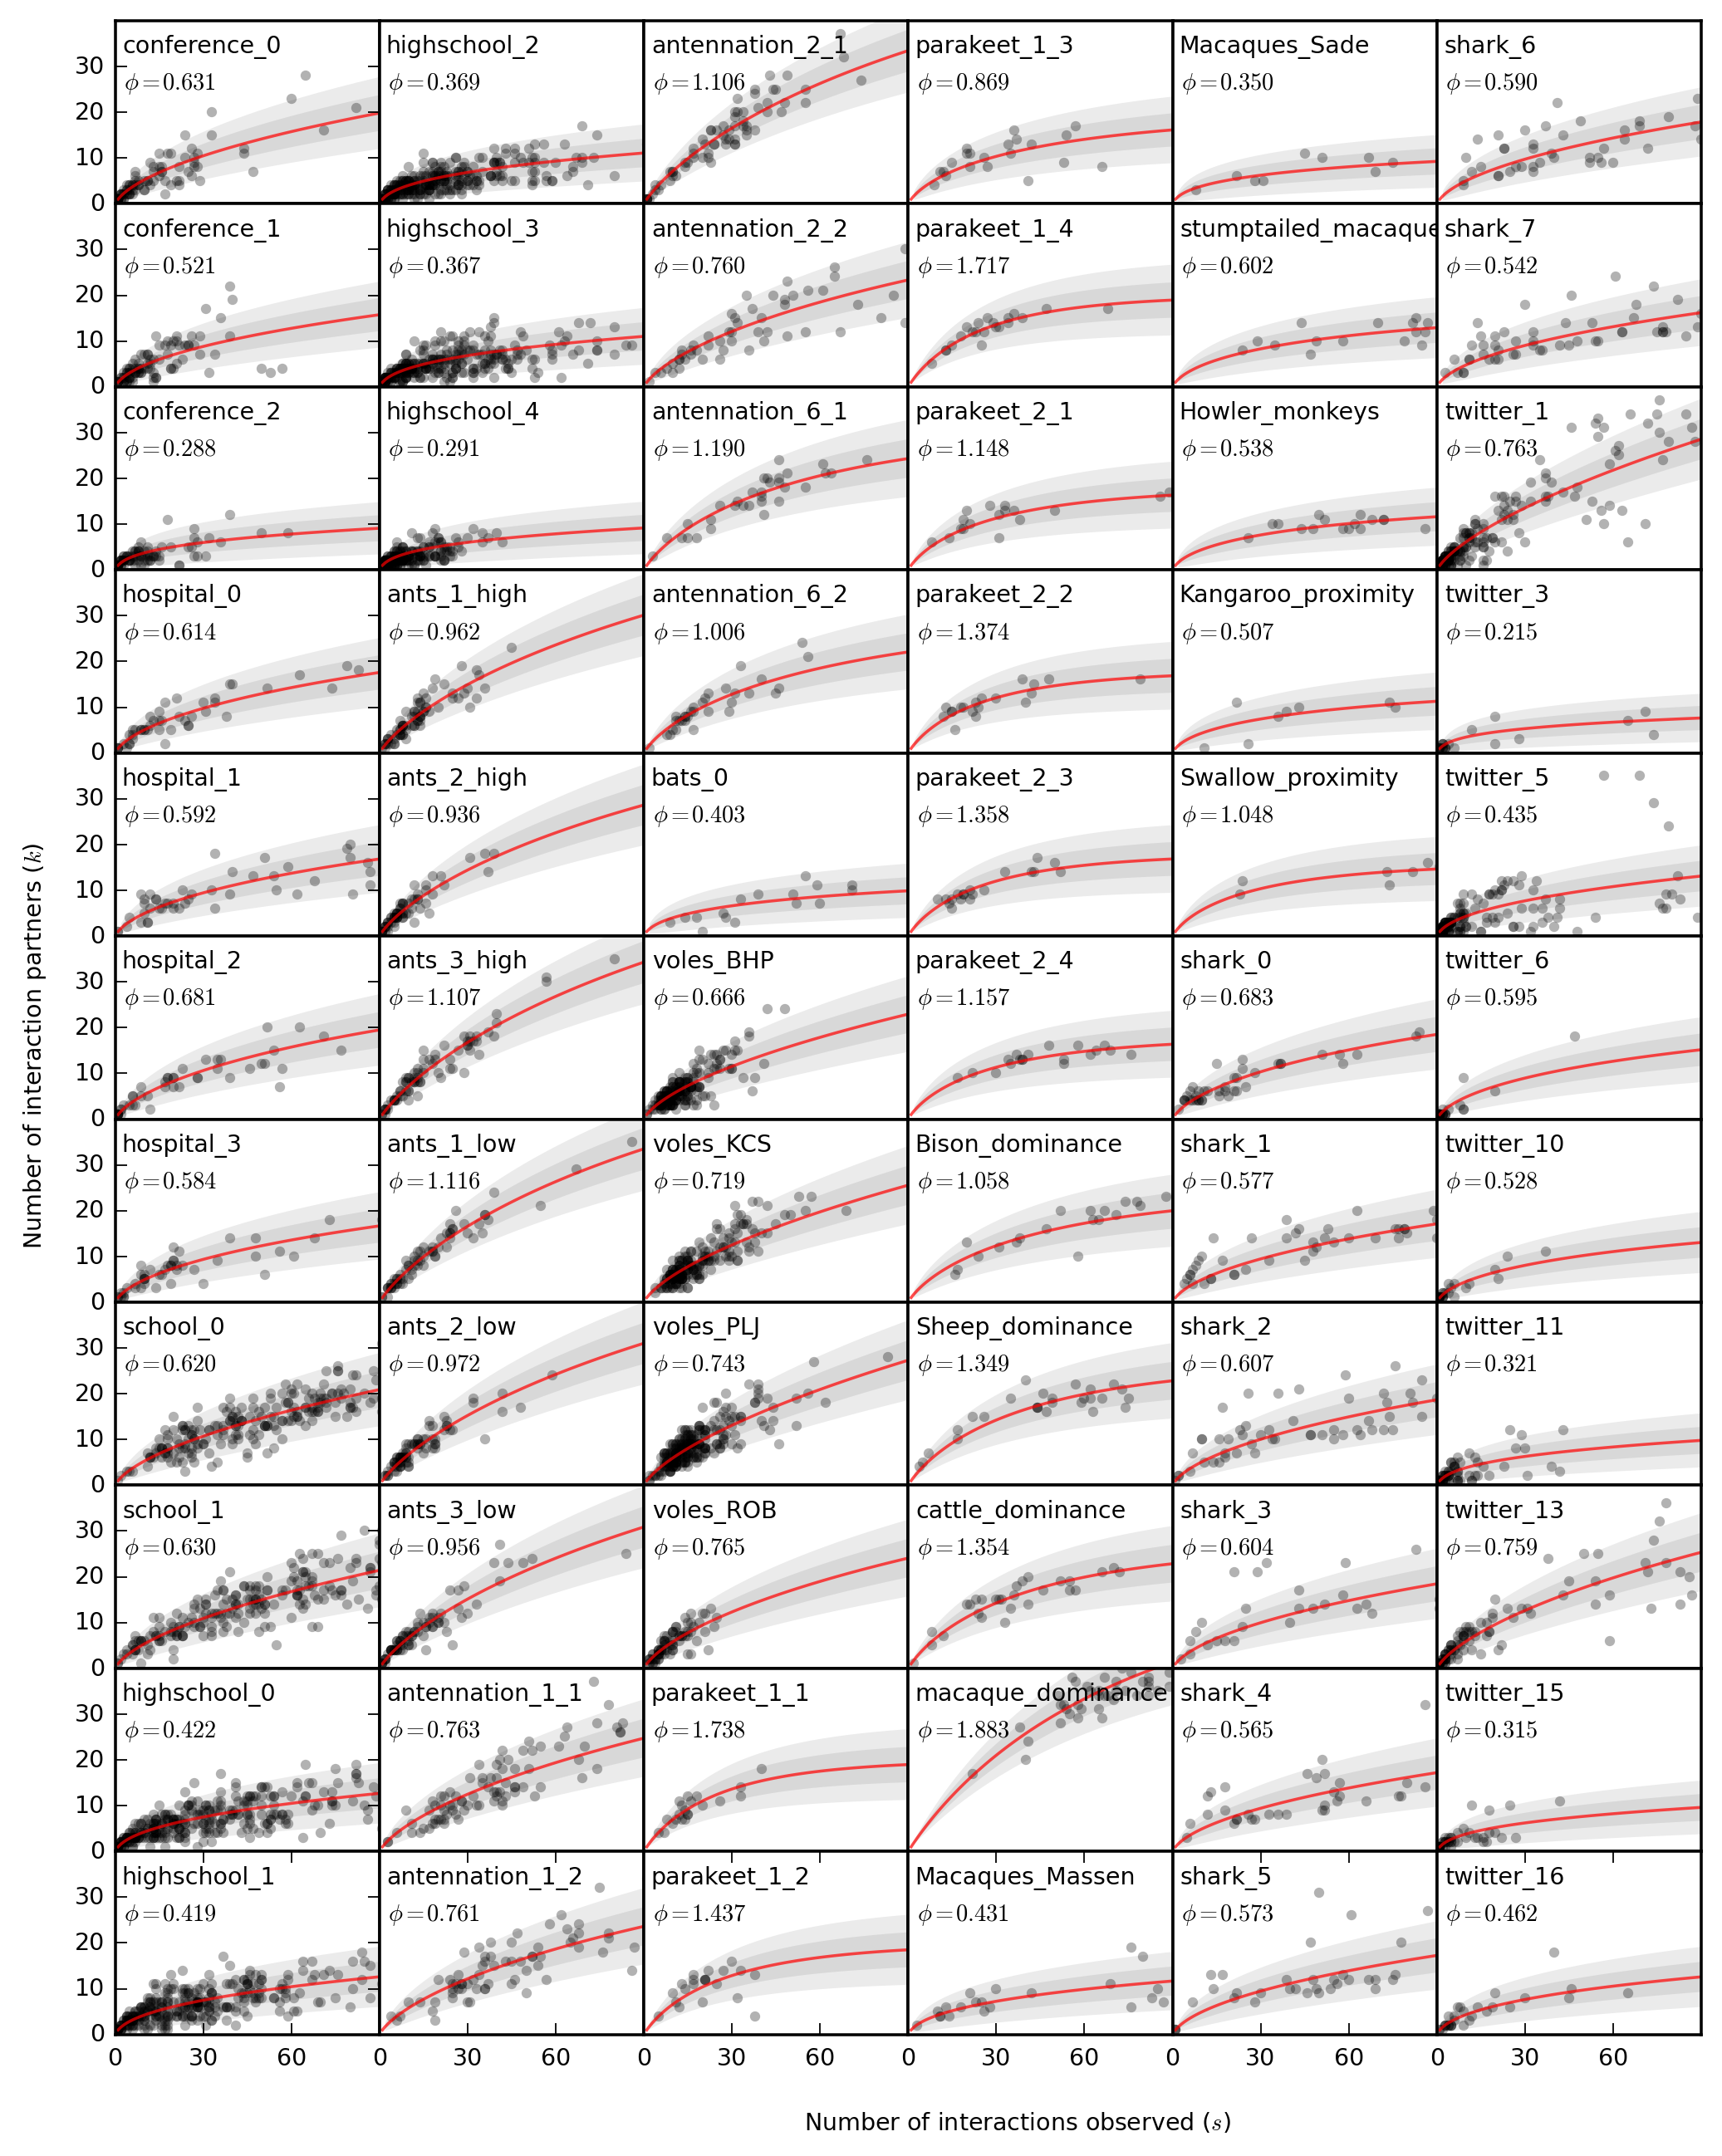
\includegraphics[width=\textwidth]{Degree_vs_int.png}
   \caption{Every data-set used in our analysis as detailed in Section \ref{data}. Each point represents one individual in the system. In each case, the mixing parameter $\phi$ has been tuned to maximize the likelihood of the model using the process described in Section \ref{fitting}. The optimal $\phi$ is given and the curve shows the mean degree of an individual as a function of the number of interactions. The shaded area and the lighter shaded area represent intervals that are one and two standard deviations from the mean respectively. Data points for which the number of interactions is more than $90$ are excluded from the figure but not from the inference of $\phi$. 
	Reference the formulas that are in the text.}
\label{Degree_vs_int}
\end{figure*}

\begin{figure*}[t]
\label{phi_vs_r}
\centering
	\includegraphics[width=0.48\textwidth]{phi_vs_r.png}\qquad
\includegraphics[width=0.48\textwidth]{f_vs_e.png}	
   \caption{Disease outcomes regarding $r_{i}$, the number of secondary infections caused by an individual $i$. On the left hand side each data point represents one of the systems in the study. The value of the mixing parameter $\phi$ (as per MLE) with error bars at one standard error, is plotted against the mean $r_{i}$ over all individuals $i$ in the population (expected values of $r_{i}$ based on $10^{3}$ simulations) with error bars showing one standard error. On the right hand side each point represents one system in the study. Those which have negative model fidelity are omitted from the plot on the left. As agreement between the model and the data (given by Eq.\eqref{fidelity}) increases, so does the agreement between analytical and simulated disease outcomes (given by the total absolute error).}
	\label{disease_fig}
\end{figure*}



\subsection{Social behavior}
\label{social_mixing}
Our analysis concerns a closed system containing a set $\mathcal{N}$ of $N$ individuals who can interact with each other in some way. The model has only one tunable parameter which can be interpreted as both the heterogeneity of relationship strengths, and the level of mixing in the population (or population fluidity). By using maximum likelihood methods we are able to measure and compare this quantity across all of our data. 

We start by considering one focal individual $i$ and its relationship to another individual $j$. Suppose that $i$ is involved in a pairwise interaction. We define the relationship strength $x_{j|i}$, for all $j\in \mathcal{N}\setminus\{i\}$, as the probability that the interaction will be with $j$.
 
If at least one interaction has occurred between $i$ and $j$ then we say that an edge exist between them. The probability that this is the case after $t$ interactions is
\begin{equation}
\label{i_to_j}
P_{i \rightarrow j}(t)=1-(1-x_{j|i})^{t}.
\end{equation}
In order to relate our approach to network theory lets first suppose that a latent network structure exists and interactions only occur between nodes connected in this network. Let $k_{i}$ be the latent degree of $i$, i.e. each $i$ has a neighborhood $\mathcal{N}_{i}$ of $k_{i}$ neighbors that they interact with at equal rates, then $x_{j|i}=1/k_{i}$ if $j\in\mathcal{N}_{i}$ and $0$ otherwise. The observed degree, $d_{i}$, increases as $t$ increases, its expectation is $\mathbb{E}[d_{i}(t)]=k_{i}[1-(1-1/k_{i})^{t}]$. The well-mixed case is recovered when $\mathcal{N}_{i}=\mathcal{N}\setminus\{i\}$ and therefore $k_{i}=N-1$. This example does not capture the whole range of values that $x_{j|i}$ can potentially take, nor does it give a good fit to any of the data that was used for this study.

We now introduce heterogeneity into the distribution of relationship strengths to create a versatile tunable model that can be fitted to various data sources. In this model we make no assumptions about the relationship between $i$ and $j$ other than that $x_{j|i}$ is drawn from some distribution $\rho(x)$. The probability that an edge exists between $i$ and any node in the network is
\begin{equation}
\label{i_to_any}
P_{i}(t)=1-\int\rho(x)(1-x)^{t}dx.
\end{equation}
Letting $d_{i}$ be the degree of $i$, the expectation is simply $\mathbb{E}(d_{i})=(N-1)P_{i}(t)$. For a given distribution ($\rho$) of relationship strengths in a population we now have a formula that connects the number of interactions to the degree.

Our goal is to choose the distribution $\rho$ that produces an accurate recreation of the behavior seen in real social systems. We therefore choose the truncated power law,
\begin{equation}
\label{distribution}
\rho(x)=\frac{\phi\epsilon^{\phi}}{1-\epsilon^{\phi}}x^{-(1+\phi)} \text{ for } \epsilon<x<1.
\end{equation}
The reason for this choosing a power law is that it allows the heterogeneity of the relationship strengths to be controlled by a single parameter $\phi$ making it adaptable to a wide variety of social systems. The distribution is truncated at $\epsilon$ so as not to include an asymptote at $x=0$. It is truncated $1$ to ensure that all values of $x_{j|i}$, which are probabilities, are less than $1$.

The value of $\epsilon$ is determined by the choice of $\phi$. To find $\epsilon$, consider that interactions are pairwise; when $i$ interacts, exactly one other individual is involved. Hence, the expectation of the sum of the $x_{j|i}$'s over all $j\in \mathcal{N}\setminus\{i\}$ is equal to $1$. Another way to express this is
\begin{equation}
\label{sum_of_x}
(N-1) \langle x \rangle = 1
\end{equation}
where $\langle x \rangle$ denotes the mean of the distribution $\rho(x)$, and is
\begin{equation}
\label{x_mean}
\langle x \rangle=\frac{\phi\epsilon^{\phi}(1-\epsilon^{1-\phi})}{(1-\phi)(1-\epsilon^{\phi})}.
\end{equation}
Combining Eq.\eqref{sum_of_x} and Eq.\eqref{x_mean} we find that the only possible choice of $\epsilon$ is the solution of
\begin{equation}
\label{epsilon}
(A+1)\epsilon^{\phi}-\epsilon-A=0
\end{equation}
where $A=(1-\phi)/(N-1)\phi$. The solution of Eq.\eqref{i_to_any} is
\begin{equation}
\label{hyper_solution}
P_{i}(t)=1-\frac{\phi\epsilon^{\phi}(1-\epsilon)^{t+1}}{(1-\epsilon^{\phi})(t+1)}{}_{2}F_{1}(t+1, 1+\phi, t+2, 1-\epsilon)
\end{equation}
The notation ${}_{2}F_{1}$ refers to the Gauss hypergeometric function \cite{absteg}. Recall that $P_{i}(t)$ is the probability that an edge exists from $i$ to $j$, for any $j\in \mathcal{N}\setminus\{i\}$, after $i$ has been involved in $t$ interactions. The existence of any edge is therefore determined by a Bernoulli trial independent of the existence of any other. After $t$ interactions the degree of $i$ should therefore follow a binomial distribution $d_{i}(t)\sim B(N-1,P_{i}(t))$, however, this gives non-zero probabilities for cases where $d>t$. This only occurs for $0<t<N$ so we replace the formula in this region with a binomial distribution with the same mean, $(N-1)P_{i}(t)$, but bounded by $t$. Thus 
\begin{equation}
\label{binoms} 
d_{i}(t) \sim 
   \begin{dcases}
    B\left(t,\frac{(N-1)P_{i}(t)}{t}\right) & \text{ if }0<t<N\\
    B\left(N-1,P_{i}(t))\right) & \text{ if } t \geq N
  \end{dcases}
\end{equation}
\subsection{Fitting to data}
\label{fitting}
The previous analysis is used to find the value of $\phi$ that give the best fit to the data. The model we have described is based on the assumption that the system is closed; over some sampling period the $N$ individuals only interact with others from the same population. For each node $i$ we need to know know the number of time they interacted, $t_{i}$, and the number of others they interacted with, $d_{i}$. We write this as two vectors $\textbf{d}=\{d_{1},d_{2},...,d_{N}\}$ and $\textbf{t}=\{t_{1},t_{2},...,t_{N}\}$.

The family of distributions in Eq.\eqref{binoms} allow us to calculate $P(d|t)$, the probability that an individual will have degree $d$ given that they have interacted $t$ times, for any value of the global parameter $\phi$. The log-likelihood function is
\begin{equation}
\log \mathcal{L}(\phi|\textbf{d},\textbf{t})=\sum_{i=1}^{N}\log[P(d_{i}|t_{i})].
\end{equation}
We then compute the maximum likely estimate of $\phi$, $\phi=\text{argmax}_{\phi}\log \mathcal{L}(\phi|\textbf{d},\textbf{t})$. Standard error $SE_{\phi}$ is calculated at $95\%$ confidence intervals using $SE_{\phi}=1.96/\sqrt{-N(\log \mathcal{L})''}$ where the derivatives of $\log \mathcal{L}$ are computed numerically. The standard error is a measure of confidence that our chosen $\phi$ is in fact the best choice. It does not tell us how well the model fits the data in the first place. To quantify this we introduce a measure of model fidelity.

To measure model fidelity we compare the likelihood of the proposed model it to a null model that represents the most random, i.e. uniformly distributed, possible degree distribution for each given $t$. The null model equivalent of Eq.\eqref{binoms} is
\begin{equation}
\label{uniforms} 
d_{i}(t) \sim 
   \begin{dcases}
    U(0,t) & \text{ if }0<t<N\\
    U(0,N-1) & \text{ if } t \geq N.
  \end{dcases}
\end{equation}
Model fidelity, $f_{\phi}$, quantifies the amount to which the proposed model fits the data when compared to an equivalent null model. We define it as
\begin{equation}
\label{fidelity}
f_{\phi}=(1/N)[\log \mathcal{L}(\phi|\textbf{d},\textbf{t})-\log \mathcal{L}(\text{null}|\textbf{d},\textbf{t})].
\end{equation}
Because we are using observed values of $t_{i}$ this approach controls for fact activity levels may vary between data sets.
%%%%%%%%%%%%%%%%%%%%%%%%%%%%%%%%%%%%%%%%%%%%%%%%%%%%%%%%%%%%%%%%%%%%%%%%%%%%%%%%%%
\begin{table*}[t] 
\centering
\caption{Summary of parameters and variables}
\label{results}
\begin{tabular}{|c||c|}
\toprule
Social behavior & Disease transmission\\
\midrule
\begin{tabular}{r|p{7cm}}
 & \\
 $N$ & Number of nodes \\
$\sum t_{i}$ & The total number of interactions of all nodes \\
$\phi$ & The mixing parameter. The optimal value calculated from the process described in Section \ref{social_mixing} \\
$\epsilon$ & The lower cut-off for the relationship strength distribution, Eq.\eqref{distribution} \\
$SE_{\phi}$ & The standard error of the estimate of $\phi$ \\
$f_{\phi}$ & Model fidelity. Given by Eq.\eqref{fidelity} \\
 & \\
\end{tabular}
&
\begin{tabular}{r|p{7cm}}
$\beta$ & The probability of transmission given that contact has occurred\\
 $\gamma$ & Recovery rate of the disease model. Chosen so that the mean number of infectious contacts is the same across all data-sets Eq.\eqref{gamma}\\
$\bar{r}$ & Mean individual reproduction number based on disease simulation.\\
$SE_{r}$ & Standard error of the reproduction number based on disease simulation\\
$|e|$ & Absolute error. Sum of the differences between $r_{i}$ predicted by Eq.\eqref{r_i} and $r_{i}$ simulated \\
\end{tabular}\\
\bottomrule
\end{tabular}
\end{table*}
%%%%%%%%%%%%%%%%%
\vspace{2cm}
%%%%%%%%%%%%%%%%%%%%%%%%%%%%%%%%%%%%%
\subsection{Disease transmission}
\label{disease_section}
Modeling the effect of $\phi$ on the number of secondary infections
We derive the expectation of the number of secondary infections caused by one infectious individual in the population. We shall refer to that individual as $i$. We will assume that the disease in question follows SIR dynamics according to the following parameters:
\begin{center}
\begin{tabular}{c|l}
$a_{i}$& Contact rate of $i$\\
$\phi$& Mixing parameter\\
$\gamma$& Recovery rate\\
$\beta$ & Transmission probability
\end{tabular}
\end{center}
If $i$ is infectious for a time period of length $\tau$ then the probability that the infection has spread from $i$ to any other individual $j$ is equal to the probability that at least one contact that occurred in that time was infectious. Since contact between individuals follows a Poisson process with rate $a_{i}$, and each contact is infectious with probability $\beta$, this is
\begin{equation}
T_{i\rightarrow j}(\tau,a_{i},x_{j|i})=1-\exp(a_{i}x_{j|i}\beta\tau) 
\end{equation}
As in Section \ref{social_mixing} we make no assumptions about the relationship between $i$ and $j$ other than that $x_{j|i}$ is drawn from the distribution given by Eq.\eqref{distribution}. The probability that transmission occurs from $i$ to any other node in the network is
\begin{equation}
\label{with_tau}
\begin{split}
T_{i}(\tau,a_{i})&=\int_{0}^{\infty}\rho(x)T_{i\rightarrow j}(\tau,a_{i},x)dx\\
&=1-\frac{\phi\epsilon^{\phi}}{1-\epsilon^{\phi}}\int_{\epsilon}^{1}x^{-(1+\phi)}\exp(a_{i}x_{j|i}\beta\tau)dx\\
&=1-\phi\sum_{k=0}^{\infty}\frac{(-a_{i}\beta\tau)^{k}}{(k-\phi)k!}\frac{\epsilon^{\phi}-\epsilon^{k}}{1-\epsilon^{\phi}}.
\end{split}
\end{equation}
Since the rate at which infected individuals move from the infected state (I) to the recovered state (R) is constant, the time spent in the infectious period follows an exponential distribution. In other words the probability that an individual spend a duration $\tau$ in the infectious state is $\gamma\exp(-\gamma\tau)$. Integrating Eq.\eqref{with_tau} across all possible values of $\tau$ we get
\begin{equation}
\label{without_tau}
\begin{split}
T_{i}(a_{i})&=\int_{0}^{\infty}\gamma e^{-\gamma\tau}T_{i}(\tau,a_{i})d\tau\\
&=1-\phi\sum_{k=0}^{\infty}\frac{(-a_{i}\beta/\gamma)^{k}}{k-\phi}\frac{\epsilon^{\phi}-\epsilon^{k}}{1-\epsilon^{\phi}}.
\end{split}
\end{equation}
The quantity $T_{i}$ is the probability that $i$ will infect $j$ for any $j\in\mathcal{N}\setminus\{i\}$. To get the expected number of secondary infections that come from $i$ we simply have to multiply by the number of susceptibles, which is the entire population minus $i$. We call this the individual reproduction number $r_{i}$, not to be confused with the basic reproduction number $R_{0}$ which is usually reserved for use as a population level statistic. The individual reproduction number, $r_{i}(a_{i})$, is a function of the rate of contact of the individual. We have that $r_{i}(a_{i})=(N-1)T_{i}(a_{i})$; it is not possible to express $T_{i}(a_{i})$ in terms of $N$, however, we can express $N$ in terms of $\epsilon$ which we know from Eq.\eqref{epsilon} decreases as $N$ increases. Using $N-1=1/\langle x \rangle$ and Eq.\eqref{x_mean}
\begin{equation}
\label{r_i}
\begin{split}
r_{i}(a_{i})&=\frac{T_{i}(a_{i})}{\langle x \rangle}\\
&=\frac{1-\phi}{\phi(\epsilon^{\phi}-\epsilon)}\left[1-\epsilon^{\phi}-\phi\sum_{k=0}^{k=\infty}\frac{(-a_{i}\beta/\gamma)^{k}}{k-\phi}(\epsilon^{\phi}-\epsilon^{k})\right]
\end{split}
\end{equation}
which can also be expressed using hypergeometric functions
\begin{equation}
\label{with_N}
\begin{split}
r_{i}(a_{i})=&\frac{1-\phi}{\phi(\epsilon^{\phi}-\epsilon)}\left[1-\epsilon^{\phi}+\epsilon^{\phi}{}_{2}F_{1}(-\phi,1,1-\phi;-a_{i}\beta/\gamma)\right.\\
&\left.-{}_{2}F_{1}(-\phi,1,1-\phi;-\epsilon a_{i}\beta/\gamma)\right]
\end{split}
\end{equation}
Noting that the taking the limit in Eq.\eqref{r_i} as $\epsilon\rightarrow 0$ is equivalent to  $N\rightarrow \infty$ we can also say
\begin{equation} 
\label{big_N}
\lim_{N\rightarrow\infty}r_{i}(a_{i}) =\frac{1-\phi}{\phi}[-1+{}_{2}F_{1}(-\phi,1,1-\phi;-a_{i}\beta/\gamma) 
\end{equation}
if $\phi<1$ and 
\begin{equation}
\label{big_N2}
\lim_{N\rightarrow\infty}r_{i}(a_{i}) =a_{i}\beta/\gamma 
\end{equation}
if $\phi>1$ (at $\phi=1$, $\rho(x)$ is not defined). Arriving at this solution requires the use of L'Hopital's Rule.

\begin{Figure}
 \centering
 \includegraphics[height=4.6cm]{N_vs_r.png}
	\includegraphics[height=4.6cm]{phi_vs_r_limit.png}
 \captionof{figure}{Plot of Eq.\eqref{with_N}. As population size increases the expected number of secondary infections converges to the value given by Eqs.\eqref{big_N} and \eqref{big_N2}. This value increases with $\phi$ up to $\phi=1$ and then saturates. The rate of convergence, however, continues to increase. \label{N_vs_r}}
\end{Figure}

\subsection{Disease simulation}
Because the fidelity of the social behavior model, i.e. the extent to which it agrees with the data, varies across the different social settings, we expect that the predictions made in Section \ref{disease_section} are only applicable to a some of our data-sets. To test how accurate the prediction of Eq.\eqref{with_N} is, we simulated the effects of transmission on the real contact data.

The collection of data-sets we are comparing is diverse, and social activity happens on dramatically different time-scales. To control for this variability the recovery rate $\gamma$ is adjusted. We choose $\gamma$ to be  
\begin{equation}
\label{gamma}
\gamma=\frac{2\beta\sum t_{i}}{N \Delta_{t} s}
\end{equation}
where $\Delta_{t}$ is the duration of the time-frame of the data. Eq.\eqref{gamma} is equivalent to choosing $\gamma$ such that, if the system is well-mixed, then an individual with the mean rate of activity is expected to directly infect $s$ others. In all the results presented we set $s=2$.

For every individual, $i$, the simulated reproduction number $r_{i}^{\text{sim}}$ is found by averaging the number of successful infections caused by $i$ over $10^{3}$ simulation trials. Each trial followed the following procedure:
\begin{enumerate}
\item A time $\tau$ is chosen randomly and uniformly between the beginning and end of the time-frame of the data
\item The length of infectious period $\Delta_{I}$ is generated from an exponential distribution with rate parameter $\gamma$
\item A list $L$ of interactions that involved $i$ between time $\tau$ and $\tau+\Delta_{I}$ is generated. If $\tau+\Delta_{I}$ is beyond the time-frame of the data then interactions from the beginning of the sampling time-frame are used in place of the missing data. 
\item Each interaction in the set $L$ is removed with probability $1-\beta$ and $r_{i}$ is the number of remaining individuals $j\in\mathcal{N}\setminus\{i\}$ that have interactions in $L$ 
\end{enumerate}
This gives a reproduction number for every individual in the system. In Table \ref{results} and Figure \ref{disease_fig} we provide the mean $\bar{r}$ and standard error $SE_{r}$ over the population. 

Finally, to measure the accuracy of Eq.\eqref{with_N} we calculate the mean absolute error $|e|$. We first calculate the rate of activity $a_{i}=t_{i}/\Delta_{t}$ which, along with the associated values of $N$, $phi$, and $\epsilon$, is used in Eq.\eqref{with_N} to compute $r_{i}$. The error is given by 
\begin{equation}
|e|=\frac{1}{N}\sum_{i\in\mathcal{N}}|r_{i}-r_{i}^{\text{sim}}|
\end{equation}

\begin{table*}[t]
\caption{A description of each row header is given in table ...}
\label{results}
\centering
\begin{tabular}{c|cccccccccc}
\toprule
Data set & $N$  & $\sum t_{i}$ & $\phi$ & $\epsilon$ \small{$\times 10^{3}$} & $SE_{\phi}$ \small{$\times 10^{2}$} & $f_{\phi}$ & $\gamma $ \small{$\times 10^{4}$} & $\bar{r}$ & $SE_{r}$ & $|e|$\\
\midrule
\verb|ants_1_high| & $74$ & $496$ & $0.962$ & $2.030$ & $0.931$ & $0.450$ & $1.164$ & $1.478$ & $0.113$ & $0.135$\\
\verb|ants_2_high| & $68$ & $318$ & $0.936$ & $2.105$ & $1.237$ & $0.427$ & $0.812$ & $1.276$ & $0.125$ & $0.231$\\
\verb|ants_3_high| & $76$ & $674$ & $1.107$ & $2.752$ & $0.865$ & $0.655$ & $1.540$ & $1.590$ & $0.143$ & $0.119$\\
\verb|ants_1_low| & $70$ & $606$ & $1.116$ & $3.075$ & $0.962$ & $0.782$ & $1.503$ & $1.589$ & $0.156$ & $0.099$\\
\verb|ants_2_low| & $79$ & $547$ & $0.972$ & $1.926$ & $0.877$ & $0.626$ & $1.202$ & $1.475$ & $0.110$ & $0.124$\\
\verb|ants_3_low| & $83$ & $610$ & $0.957$ & $1.738$ & $0.776$ & $0.536$ & $1.276$ & $1.466$ & $0.138$ & $0.127$\\
\verb|conference_0| & $93$ & $663$ & $0.631$ & $0.356$ & $0.532$ & $0.221$ & $0.206$ & $1.158$ & $0.118$ & $0.188$\\
\verb|conference_1| & $92$ & $650$ & $0.521$ & $0.150$ & $0.561$ & $0.016$ & $0.204$ & $1.137$ & $0.088$ & $0.254$\\
\verb|conference_2| & $84$ & $477$ & $0.288$ & $0.005$ & $0.692$ & $0.424$ & $0.164$ & $0.870$ & $0.070$ & $0.223$\\
\verb|hospital_0| & $51$ & $778$ & $0.614$ & $0.878$ & $0.779$ & $0.769$ & $0.441$ & $1.136$ & $0.141$ & $0.138$\\
\verb|hospital_1| & $49$ & $1075$ & $0.592$ & $0.825$ & $0.741$ & $0.845$ & $0.635$ & $1.136$ & $0.129$ & $0.162$\\
\verb|hospital_2| & $51$ & $855$ & $0.681$ & $1.244$ & $0.774$ & $0.803$ & $0.485$ & $1.252$ & $0.156$ & $0.116$\\
\verb|hospital_3| & $50$ & $743$ & $0.584$ & $0.759$ & $0.802$ & $0.713$ & $0.430$ & $1.136$ & $0.138$ & $0.145$\\
\verb|school_0| & $237$ & $6420$ & $0.620$ & $0.070$ & $0.086$ & $1.245$ & $0.784$ & $1.298$ & $0.041$ & $0.145$\\
\verb|school_1| & $238$ & $6514$ & $0.630$ & $0.076$ & $0.086$ & $1.148$ & $0.792$ & $1.288$ & $0.047$ & $0.150$\\
\verb|twitter_1| & $245$ & $3135$ & $0.763$ & $0.192$ & $0.143$ & $-0.016$ & $0.370$ & $1.317$ & $0.124$ & $0.222$\\
\verb|twitter_3| & $23$ & $292$ & $0.215$ & $0.116$ & $2.553$ & $0.176$ & $0.367$ & $0.736$ & $0.196$ & $0.132$\\
\verb|twitter_5| & $195$ & $3322$ & $0.435$ & $0.010$ & $0.192$ & $0.018$ & $0.493$ & $0.832$ & $0.084$ & $0.234$\\
\verb|twitter_6| & $30$ & $70$ & $0.595$ & $2.021$ & $4.088$ & $-0.322$ & $0.068$ & $0.754$ & $0.241$ & $0.370$\\
\verb|twitter_10| & $24$ & $84$ & $0.528$ & $2.204$ & $4.512$ & $0.184$ & $0.101$ & $0.896$ & $0.209$ & $0.209$\\
\verb|twitter_11| & $72$ & $303$ & $0.321$ & $0.016$ & $0.998$ & $-0.002$ & $0.122$ & $0.821$ & $0.097$ & $0.283$\\
\verb|twitter_13| & $106$ & $1903$ & $0.759$ & $0.607$ & $0.364$ & $0.374$ & $0.519$ & $1.175$ & $0.148$ & $0.228$\\
\verb|twitter_15| & $49$ & $191$ & $0.315$ & $0.047$ & $1.678$ & $0.162$ & $0.113$ & $0.888$ & $0.120$ & $0.250$\\
\verb|twitter_16| & $32$ & $325$ & $0.462$ & $0.796$ & $1.714$ & $0.354$ & $0.294$ & $1.022$ & $0.178$ & $0.131$\\
\verb|voles_BHP| & $195$ & $1339$ & $0.666$ & $0.141$ & $0.222$ & $0.368$ & $132.051$ & $1.385$ & $0.057$ & $0.170$\\
\verb|voles_KCS| & $193$ & $1874$ & $0.719$ & $0.206$ & $0.188$ & $0.632$ & $186.728$ & $1.504$ & $0.059$ & $0.143$\\
\verb|voles_PLJ| & $233$ & $2126$ & $0.743$ & $0.183$ & $0.162$ & $0.448$ & $175.470$ & $1.524$ & $0.055$ & $0.145$\\
\verb|voles_ROB| & $77$ & $381$ & $0.765$ & $0.982$ & $0.876$ & $0.243$ & $95.155$ & $1.288$ & $0.080$ & $0.185$\\
\verb|bats_0| & $16$ & $290$ & $0.427$ & $3.105$ & $3.359$ & $0.640$ & $6.380$ & $0.645$ & $0.072$ & $0.221$\\
\bottomrule
\end{tabular}
\end{table*}

\section{Data}
\label{data}
We tested our analysis to $20$ study systems. Details of the number of nodes and total number of interactions can be seen in Table \ref{results}.

\subsection{Ant trophallaxis networks}
We collected data from three carpenter ant colonies (Camponotus Pennsylvanicus). In nature, carpenter ant foragers consume liquid food and, upon returning to the nest, regurgitate it into the mouths of their nest-mates, a process known as trophallaxis. Typically, foragers will only give food to a small number of other ants; to feed the entire colony it gets passed through a complex network of feeding interactions \cite{quevillon2015social}. Trophallaxis is also an important form of communication and a way that information about the state of the colony can be shared by all of its members \cite{greenwald2015ant,10.7554/eLife.20375}.

We placed colonies of approximately $80$ ants in a nest designed to replicate the conditions found in nature. The colony was first given a restrictive area of $65\times42$mm to live (high density) the ants were given several days to adjust before $4$ hours of trophallaxis activity was recorded. The nest was then expanded by a factor of $4$ (low density) and after another adjustment period another $4$ hours were recorded. The process was repeated for $3$ unrelated colonies.

[Something about ant diseases]
\subsection{Sociopatters human interaction networks}
We use human contact data from the Sociopatterns project (sociopatterns.org) \cite{isella2011s,10.1371/journal.pone.0073970,10.1371/journal.pone.0023176}. Participants wore radiofrequency identification sensors that detect face-to-face proximity of other participants within $1$-$1.5$ meters in $20$-second intervals. Each dataset lists the identities of the people in contact, as well as the $20$-second interval of detection. The timing and duration of contacts are known with a resolution of $20$-seconds. To exclude contacts detected while participants momentarily walked past one another, only contacts detected in at least two consecutive intervals are considered interactions.

The data we use comes from two studies: an academic conference which occurred over the course of $3$ days, which we divided into $3$ separate $24$-hour data-sets, and a primary school for which there are two days of data, which we divided into $2$ $24$-hour data-sets. 
%add hospital
[add hospital reference]
\cite{isella2011s},\cite{10.1371/journal.pone.0023176}
\subsection{Twitter mentions networks}
Mentions on Twitter act as way to send messages directly to particular individuals. Although the message is broadcast to all the followers of the  account of the sender it will appear in the inbox of the receiver and is therefore likely to be noticed. Mentions often replied to \cite{10.1371/journal.pone.0022656}. We count an interaction as a reciprocated twitter mention, i.e. the motif A$\rightarrow$B, B$\rightarrow$A is an  interaction for A. We ignore all mentions that are not followed by reciprocation i.e. the motif A$\rightarrow$B, A$\rightarrow$B, B$\rightarrow$A, B$\rightarrow$A is counted as exactly $1$ interaction for A.

In the study from which we take this data \cite{Charlton160162}, communities were first identified before their intensive data collection began. A range of community detection algorithms were used to decide which user accounts belong to the group and which do not, the goal being to find communities such that its members send messages within their community significant more than to user accounts outside the community. The $N$ individuals in the community form their own sub-population which acts somewhat like a closed system, a requisite for applying our analytical methods. 

We use the last 24 hours of activity in each of the $17$ communities. We discard those for which the number of active users (during the $24$ hour period) is either less than $20$ or more than $250$.

[Something about information transmission in social media]
\subsection{Vole contact networks} 
Data was collected from a population of wild voles (Microtus agrestis) to assess the role of space in determining the structure of social networks \cite{Davis20141004}. [Sentence about vole behavior and what an interaction is].

In each of four field sites $100$ traps were placed in a square grid covering $0.3$ hectares. Bait was put into the traps and then three days later observers would check the traps for voles, those who were found were tagged so that they could be recognized should they be caught again. During each trapping session the traps were checked on several consecutive days. If a vole is observed in a trap at any point during a trapping session then we say that they interacted with any other vole that was observed in the same trap at any point during the same trapping session. The time of the interaction is the day that the trapping session began. 

We then discard any voles that had $10$ or less interactions and all interactions in which they participated. Since the voles have a very short lifespan and cyclic fluctuations in population size we use only a sub-sample of each data-set. We chose periods of $130$ days selected at times of high activity for each of the four experiment sites.

[Something about vole diseases]
\subsection{Bat food-sharing networks}
Vampire bats share food with each other through regurgitation. In order to initiate such an event a hungry bat will lick the mouth of another bat from whom they hope to receive food. The data we use is a record of mouth-licking observations originally collected to address questions of altruism and reciprocity in bat communities \cite{Carter20122573,dryad_tg7b1}.

A population of vampire bats (desmodus rotundus) were kept captive in an enclosure. Out of the $25$ bats, $20$ were subjected to experimental treatment. In each case, the subject was removed from the enclosure and starved for $24$ hours. The observation period of $2$ hours began when the starved bat was let back into the enclosure and during this time the usual sources of food were not available. Thus, for the subject bat to feed, interaction with others was necessary. The starvation treatment and observations occurred on a different day for each bat. Some bats were tested more than once so to avoid biasing our results we select only the first day they were tested. 

[Something about bat diseases]
\section{Results} 
Humans, ants and online communities exhibit various levels of social mixing. We see from Figure \ref{Degree_vs_int} that social connectivity always increases with social activity, however, the rate at which it  increases depends on the data. By fitting a stochastic model to each data-set, we demonstrated that this is likely to be a result of the heterogeneity of contact strengths between nodes in the social network, and therefore a direct result of social mixing. The parameter $\phi$ controls heterogeneity in the model and is used to quantify the amount of mixing between members of the population.

The amount of mixing in a social system relates directly to a higher rate of disease transmission. In an otherwise fully susceptible population, the individual reproduction number $r_{i}$, the number of infections caused by an infectious individual $i$, increases with $\phi$. This is known from the results of simulating diseases with SIR dynamics, plotted in Figure \ref{disease_fig} (left), and analytically from Eq.\eqref{with_N}. For most data-sets the social behavior model does a good job of predicting $r_{i}$, however, in cases where the level of agreement between the model and the data is low, so too is its ability to predict disease outcomes (Figure \ref{disease_fig} (right)).

As the population size increases to $\infty$ the individual reproduction number converges for all values of $\phi$, however, for populations of infinite size an abrupt phase transition occurs when $\phi=1$. Below this value ($\phi<1$) mixing is low and interactions are repeated frequently enough to slow the spread of disease. Beyond this value ($\phi>1$) the probability that an interaction is repeated is $0$ and the number of infections is equal to what it would be in a mass-action model (Figure \ref{N_vs_r}).


\section{Discussion}
We have measured the level of mixing in a wide variety of social systems and explored how it affects the spread of infectious disease. We have found that disease transmission is influenced by underlying social factors, in particular, the way individuals distribute their attention among other members of the population. By using a power-law to model of heterogeneity in the distribution of contact rates, we are able to accurately reproduce the relationship between the number of interactions of individuals and their degree. 

As a tool for predicting the risks of epidemic our analysis has two appealing qualities. Firstly, no information was needed other than two basic quantities associated with social behavior, the degree and the number of interactions of each individual. Our method can therefore be applied without requiring large amounts of personal information. Secondly, The method provides a single numerical value which indicates how mixed a population is, and consequently how easy it will be for an infectious disease to spread.

We have discovered that ants are not particularly averse to the risks of infectious disease. This is not surprising; in addition to the distribution of food, ants use trophallaxis to share information, and share nutrients that are essential for the growth and well-being of the colony. In comparison the costs of infection seem insignificant and the large value of $\phi$ corroborates this. In the human data, $\phi$ seems to cluster around $1.6$. If this value is indeed indicative of typical human social behavior then we can conclude that the force of infection in the mass-action model is too high. A question which we leave unanswered is how much inaccuracy and over-prediction this leads to when assessments are made about the risks of emerging diseases. We would need consider movement patterns and social behavior over longer durations and greater distances; it should not be assumed that the heterogeneity of contact probabilities we see in localized populations is the correct model at this scale.

%the most famous result in the theory of social limitations saturation occurs once a given number of social ties, in humans this number is approximately 150, in primates it is lower, and in most species it is not known, so with more data we expect to see the curve continue to grow and then saturate around this value.  If this can be overcome then there is no reason to believe that the theory, heterogeneity of contact rates, can explain mixing phenomena on a larger scale. 

%The slow covergence to a ... that we see in Figure \ref{N_vs_r} implies that density dependence is always the case in this model. In circumstances where the model works, where model fidelity is high, we can conclude that the system with respect to a particular definition of transmisible contact is density depenent albeit in a non-linear way. 

Additionally, we should not expect mixing to remain constant across time, particularly as culture changes and social norms shift. If mixing were to increase in terms of sexual contact, for example, a small change in $\phi$ could be the catalyst for an endemic sexually transmitted disease to become an epidemic. Likewise, as transportation of livestock becomes more efficient, animals can be moved over larger distances and at greater speed, potentially increasing the mixing and allowing new strains of airborne disease to emerge.

Mixing in an animal population or human society is a variable that can be quantified. Having the ability to summarize large amounts of complexity with one number will improve our ability to understand, and communicate, the risks associated with infectious disease.

\end{multicols}
\small
\bibliography{bibfile}
\bibliographystyle{ieeetr}
\normalsize

\end{document}
